
\subsubsection{Caso d'uso UC8.2 - Procedura di Acquisto API}
\label{UC8.2}
\begin{figure}[ht]
	\centering
	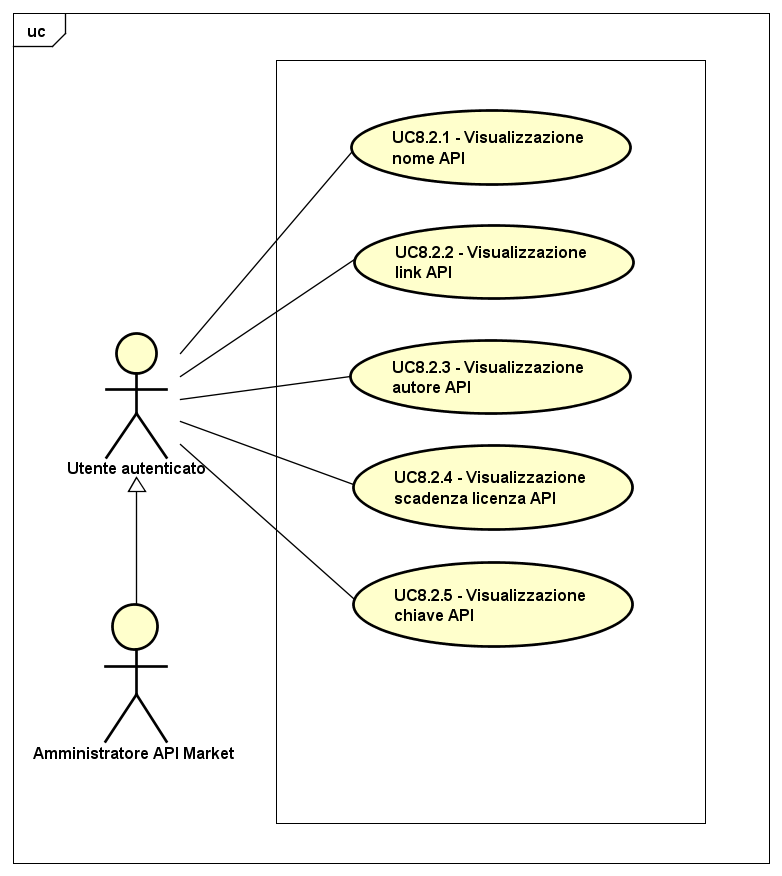
\includegraphics[scale=0.45]{UML/UC8_2.png}
	\caption{UC8.2 - Procedura di Acquisto API}
\end{figure}
\FloatBarrier
\begin{longtable}{ l | p{11cm}}
	\hline
	\rowcolor{Gray}
	\multicolumn{2}{c}{UC8.2 - Procedura di Acquisto API}\\
	\hline
	 \textbf{Attori} & Utente autenticat, Amministratore APIMarket, Sistema \\
	\textbf{Descrizione} & L'utente puo' comprare un'API e puo' farlo in diversi modi, anche secondo una procedura esterna (un esempio di procedura esterna e' Paypal)\\
	\textbf{Pre-Condizioni} & L'utente ha selezionato un'API\\
	\textbf{Post-Condizioni} & L'utente ha acquistato l'API e ricevuto la chiave API associata\\
	\textbf{Scenario Principale} & 
	\begin{enumerate*}[label=(\arabic*.),itemjoin={\newline}]
		\item L'utente puo' scegliere il Piano di Acquisto(UC8.2.1)
		\item L'utente puo' scegliere la modalita' di Acquisto (UC8.2.2)
		\item L'utente puo' confermare l'Acquisto (UC8.2.3)
		\item L'utente puo' Visualizzare l'Errore di Acquisto (UC8.2.4)
		\item L'utente puo' confermare l'Acquisto Avvenuto (UC8.2.5)
		\item Il sistema puo' eseguire l'Acquisto usando una procedura d'Acquisto esterna (UC8.2.6)
		\item L'utente puo' ricevere una Chiave API dopo l'Acquisto (UC8.2.7)
	\end{enumerate*}\\
	\textbf{Scenari Alternativi} & 
	\begin{enumerate*}[label=(\arabic*.),itemjoin={\newline}]
		\item L'utente puo' Visualizzare l'Errore di Acquisto (UC8.2.4)
	\end{enumerate*}\\
\end{longtable}
